In this section, we show that for every partly \textsc{EviL} Kripke
structure, we may ``complete'' it by constructing a bisimilar
\textsc{EviL} structure; this amounts to enforcing the \textsc{EviL} property \ref{pVII},
namely that a world is reflexive for $R_X$ if and only if it models
$\PP_X$.  This will allow us to establish that \textsc{EviL} is sound
and strongly complete for \textsc{EviL} Kripke models.

We shall first review the definition of \emph{bisimulation}, which we
shall have to modify somewhat given our modified definition of Kripke
structures.  We follow \cite[Definition 2.16, pg.
64]{blackburn_modal_2001} in our presentation:

\begin{mydef}\label{bisimdef}
Let $\mathbb{M} = \langle W, R, \sqsubseteq, \sqsupseteq, V, P
\rangle$ and $\mathbb{M}' = \langle W', R', \sqsubseteq',
\sqsupseteq', V', P' \rangle$.
A non-empty binary relation $Z \subseteq W \times W'$ is a called a
\textbf{bisimulation between $\mathbb{M}$ and $\mathbb{M}'$} (denoted
$Z: \mathbb{M} \leftrightarroweq \mathbb{M}'$) if the following are
satisfied:
\begin{myroman}
  \item If $wZw'$ then $w$ and $w'$ satisfy the same proposition
    letters, along with the special letters $P_X$.
  \item \textbf{Forth} --   
    If $wZ w'$ and $w \leadsto v$, then there exists a $v' \in W'$ such that
    $v Z v'$ and $w' \leadsto' v'$.  
\item \textbf{Back} -- If $wZ w'$ then $w'\leadsto' v'$, then there exists a $v \in W$ such
    that $v Z v'$ and $w \leadsto v$.
\end{myroman}
\ldots where $\leadsto$ is any of $R_X$, $\sqsubseteq_X$, or
$\sqsupseteq_X$, where $X$ is any agent in the class of agents $\mathcal{A}$.
\end{mydef}

We now recall one of the most crucial theorems in all of modal logic:
\begin{theorem}[The Fundamental Theorem of Bisimulations]\label{fundamental-bisim-theorem}
If $Z: \mathbb{M} \leftrightarroweq \mathbb{M}'$ and $w Z w'$, then
for all formulae $\phi$ we have that $$\mathbb{M}, w \Vdash \phi
\textup{ if
and only if }\mathbb{M}', w' \Vdash \phi$$
\end{theorem}
\begin{proof}
This is Theorem 2.20 in \cite[pg. 67]{blackburn_modal_2001}
\end{proof}

We now  introduce a Backus-Naur form grammar for the
$\mathsf{Either}$ type constructor. This will give us precise notation
for manipulating the disjoint union of a Kripke structure $\mathbb{M}$
with itself.

\begin{mydef}\label{eitherdef}
\[ \mathsf{Either}\ a\ b ::= a_l \ |\ b_r \]
\end{mydef}

We now make use of this grammar to express an operation for making bisimilar models:

\begin{mydef}[Bisimulator]
Let $\mathbb{M}$ be a Kripke model, then define a new Kripke model:
$$\invis^\mathbb{M} := \langle W^{\invis}, R^{\invis}, \sqsubseteq^{\invis},
\sqsupseteq^{\invis}, V^{\invis}, P^{\invis} \rangle$$ 
%  as a model
% \[\la W^{\invis^\mathbb{M}},V^{\invis^\mathbb{M}}, P^{\invis^\mathbb{M}}_X,R^{\invis^\mathbb{M}}_{\Nec_X},R^{\invis^\mathbb{M}}_{\BB_X},R^{\invis^\mathbb{M}}_{\BBI_X}\ra\] 
where:
 \begin{eqnarray*}
 W^\invis & := &  \{w_l,w_r\ |\ w\in W^{\mathbb{M}} \} \\
 V^\invis(p) & := &  \{w_l,w_r\ |\ w\in V^{\mathbb{M}}(p)\}\\
 P^\invis_X & := &  \{w_l,w_r \ |\  w\in P^\mathbb{M}_X\}\\
 R^\invis_X & := &  \{(w_l,v_r),(w_r,v_l)\ |\ w R^\mathbb{M}_X v \} \cup \\
 & & \{(w_l,v_l), (w_r,v_r) \ |\ w R^\mathbb{M}_X v
\  \&\  w \in P^\mathbb{M}_X\} \\
 \sqsupseteq_X^\invis & := & \{(w_l,v_l),(w_r,v_r)\ | \ 
 w \sqsupseteq^\mathbb{M}_X v \} \\
 \sqsubseteq_X^\invis & := & \{(w_l,v_l),(w_r,v_r)\ | \ 
 w \sqsubseteq^\mathbb{M}_X v \} 
 \end{eqnarray*}
\end{mydef}

It is instructive to review how $\invis$ operates on
Kripke models it takes as input.  
One idea is that $\invis$ causes every world $w$ in
$\mathbb{M}$ to undergo \emph{mitosis}, and split into two identical
copies named $w_l$ and $w_r$.  These copies obey three rules:
\begin{mynum}
\item The \emph{left copy} of a world $w$, denoted $w_l$, can see
  the \emph{right copy} of a world $v$, denoted $v_r$, provided that
  $w R^\mathbb{M} v$ originally.  This is similarly true for right
  copies, only reflected. 
\item If $\mathbb{M}, w \Vdash \PP_X$, then the copies $w_l$ and $w_r$
  of $w$ can see both $v_l$ and $v_r$ provided that $w R^\mathbb{M} v$
  to begin with.
\item If $w \sqsubseteq_X^\mathbb{M} v$ then
$w_l \sqsubseteq_X^\invis v_l$ and $w_r \sqsubseteq_X^\invis v_r$, but
never $w_l \sqsubseteq_X^\invis v_r$ or $w_r \sqsubseteq_X^\invis
v_l$.
\end{mynum}

The reason $\invis$ duplicates everything in this manner is because
we are preventing $R_X$ reflexivity whenever $w \nin P_X$.
This means that when $w R^\mathbb{M} v$, there are two situations,
which are depicted in Figs. \ref{fig:bisim1} and \ref{fig:bisim2}.
The third rule is depicted in \ref{fig:bisim3}.

For clarity, here is how one should read these three diagrams:
\begin{bul}
 \item If one point $w$ is connected to another point $w'$ by a
   dotted lines with arrows at both ends 
   \tikz \draw[<->,>=latex, dotted ,semithick](0pt,0pt) -- (20pt,6pt);, then
   those points are bisimilar.
 %  this means that $a = b$ and $B \subset A$.
  \item If one point $w$ is connected to another point $v$ by
    a solid line with an arrow and a label $X$ \tikz
    \draw[](0pt,0pt) edge[->,>=latex,semithick] node[xshift=-2.5pt,yshift=-1pt,fill=white,inner sep=.5pt] {\tiny $X$}
    (20pt,6pt) ;, then $w R_X v$, taking care to note which model we are
    reasoning in.
  \item If one point $w$ is connected and \emph{above} to another point $v$ by
    a densely line with no arrow and a label $X$ \tikz
    \draw[](0pt,0pt) edge[densely dotted, semithick] node[fill=white,inner sep=.5pt] {\tiny $X$}
    (20pt,6pt) ;, then $w \sqsupseteq_X v$. 
\end{bul}

\begin{figure}[ht]
\centering
\subfigure[$\mathbb{M},w\Vdash \PP_X$]{
  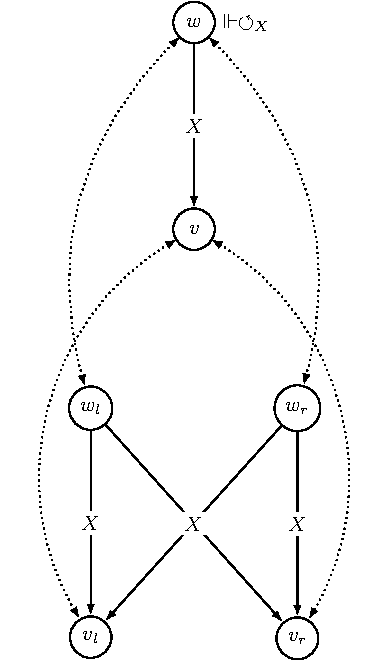
\includegraphics[height=.4\textheight]{evil_pictures/bisim1.pdf}
%\caption{A fairly simple example}
\label{fig:bisim1}
}
\subfigure[$\mathbb{M},w\nVdash \PP_X$]{
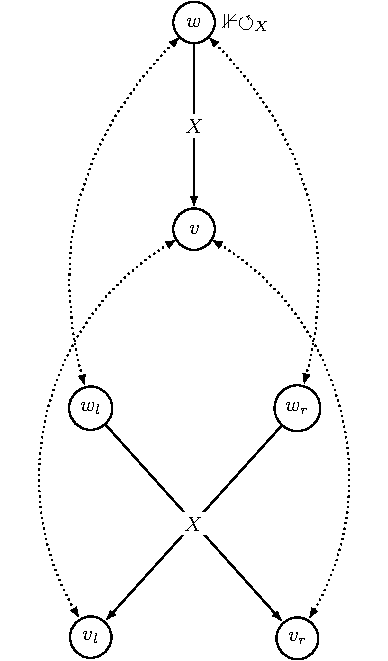
\includegraphics[height=.4\textheight]{evil_pictures/bisim2.pdf}
\label{fig:bisim2}
} 
\subfigure[Always]{
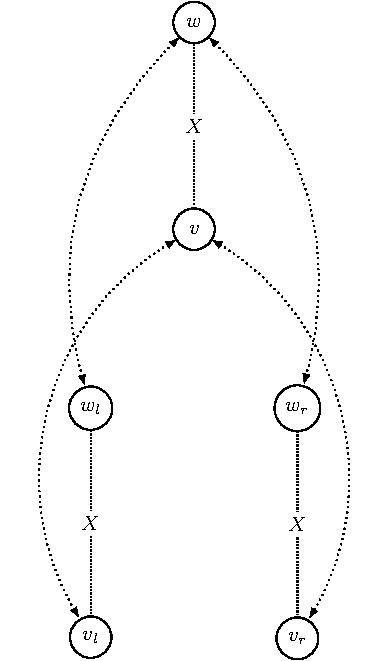
\includegraphics[height=.4\textheight]{evil_pictures/bisim3.pdf}
\label{fig:bisim3}
}

\caption{Visualizations of $\invis$'s operation}
\end{figure}

We summarize the mechanics of $\invis$ in the following proposition:
\begin{proposition}\label{inviskey}
Let $\{w, v\}\subseteq W^\invis$, and let $\{w^\circ, v^\circ\}
\subseteq W^\mathbb{M}$ such that $w^\circ_l = w$ or $w^\circ_r = w$
and similarly for $v^\circ$.
\begin{mynum}
\item If $w$ and $v$ have different handedness, then
\begin{eqnarray*}
&w R^\invis_X v\textup{ if and only if } w^\circ R^\mathbb{M}_X
v^\circ \\
& \& \\
&w \sqsubseteq^\invis_X v\textup{ or }v \sqsubseteq^\invis_X w  \textup{ never holds}
\end{eqnarray*}
\item If $w$ and $v$ have the same handedness, then 
\begin{eqnarray*}
&w R^\invis_X v \textup{ if and only if } w \in
P_X^\mathbb{M}\ \& \ w^\circ R^\mathbb{M}_X v^\circ \\
& \& \\
&w \sqsubseteq^\invis_X v\textup{ if and only if }  w^\circ \sqsubseteq^\mathbb{M}_X v^\circ 
\end{eqnarray*}
\end{mynum}
\end{proposition}

We shall now provide proof that $\invis$ gives rise to a bisimulation:

\begin{lemma}\label{bisimulation}
For any Kripke model $\mathbb{M} = \la W,V,P_X,R_{\Nec_X},R_{\BB_X}, R_{\BBI_X}\ra$, we have the following bisimulation $Z: \mathbb{M} \leftrightarroweq \invis^\mathbb{M}$:
\begin{eqnarray*} w Z w_l & \& & w Z w_r \end{eqnarray*}
\end{lemma}
\begin{proof}
  It follows directly from the definition of $\invis$ that the truth
  of the letters are preserved, along
  with the back and forth conditions for the $\sqsubseteq_X$ and
  $\sqsupseteq_X$ relations.  The proof of the back and forth
  conditions for $R_X$ involves elementary reasoning by cases on whether
  $\mathbb{M}, w \Vdash \PP_X$ or not. This simple argumentation 
  suffices the rest of the proof.
\end{proof}

We now turn to proving that this bisimulation completes a partially
\textsc{EviL} Kripke structure. We shall make use the mechanics of the 
 construction of $\invis$ heavily.

\begin{theorem}[\textsc{EviL} Completion]\label{EviL-Completion}
If $\mathbb{M}$ is partly \textsc{EviL} Kripke structure then
$\invis^\mathbb{M}$ is an \textsc{EviL} Kripke structure. 
\end{theorem}
\begin{proof}
We must verify that $\invis^\mathbb{M}$ makes true all of the
\textsc{EviL} properties.  We may observe that \ref{pI} through
\ref{pislandiff} and \ref{pVI} follow by construction, and 
the fact that since
$\mathbb{M}$ is partly \textsc{EviL} by hypothesis it makes true \ref{ppI} through
\ref{islandiff} and \ref{ppVI}.  All that is left to show is \ref{pV}
and \ref{pVII}.

  \begin{description}
    \item[\ref{pV}] We must show
$$(R^{\invis}_X \circ \sqsubseteq^{\invis}_X) \subseteq
    R^{\invis}_X \subseteq (R^{\invis}_X \circ
    \sqsupseteq^{\invis}_X)$$
Since we already know that $\sqsubseteq^\invis$ is the reverse of
$\sqsupseteq^\invis$, it suffices to show that $(R^{\invis}_X \circ
\sqsubseteq^{\invis}_X) \subseteq   R^{\invis}_X$.  
So assume that $w  \sqsubseteq^{\invis}_X u$ and $u R^{\invis}_X v$. We know that since $w \sqsubseteq^{\invis}_X u$ then by construction
they must have the same handedness.  Without loss of generality assume
that both $w$ and $u$ are \emph{left}, that is there is some
$\{w^\circ,u^\circ\} \subseteq W^\mathbb{M}$ such that $w = w^\circ_l$
and $u = u^\circ_l$. By construction we have that $w^\circ
\sqsubseteq^\mathbb{M} u^\circ$.  It suffices to show that $w R_X^\invis
v$; to do this we shall reason by cases on the handedness of $v$.
  \begin{description}
\item[Opposite --] Assume that $v$ has the opposite handedness, hence $v = v^\circ_r$ for
some $v^\circ\in W^\mathbb{M}$. Then by construction we have that
$u^\circ R_X^\mathbb{M} v^\circ$.  This means that since
$\mathbb{M}$ is partly \textsc{EviL}, it makes true \ref{ppV}, so $w^\circ
R_X^\mathbb{M} v^\circ$.  Hence by construction we have $w R^\invis_X v$.
\item[Same --]  Now assume that $v$ has the same handedness as $w$ and
  $u$, so $v = v^\circ_l$ for some $v^\circ\in W^\mathbb{M}$.  Since
  $u^\circ_l R^\invis_X v^\circ_l$ by assumption, we know from the
  definition of $\invis$ that $u^\circ \in P_X^\mathbb{M}$.  Since
  $\mathbb{M}$ is partly \textsc{EviL} by hypothesis, and $u
  \sqsupseteq_X w$, then from \ref{ppIX} we have that $w \in
  P_X^\mathbb{M}$.  But then we know by \ref{ppV} that $w^\circ
  R^\mathbb{M}_X v^\circ$, hence by construction we have
   $w R^\invis_X v$ as desired.
\end{description}

\item[\ref{pVII}]  We must show that ``$w \in P_X^\invis$ if
  and only if $w \sqsupseteq^\invis_X w$''. We know that the
  left to right direction holds by construction, since by assumption
  $\mathbb{M}$ is partly \textsc{EviL} and hence makes true
  \ref{ppVII}.

  Now assume that  $w \sqsupseteq^\invis_X w$, then since $w$ can see
  something with the same handedness as itself (namely itself), 
by construction we know that $w^\circ \in P_X^\mathbb{M}$ where $w^\circ_l = w$ or
$w^\circ_r=w$.  Whence $w \in P^\invis_X$, which completes the argument.
\end{description}
\end{proof}

With these observations, we may now strengthen Theorem
\ref{partly-evil-completeness} from partly \textsc{EviL} models to
the fully \textsc{EviL} models originally defined in
Definition \ref{evil-kripke-structures} from \S\ref{kripke}:

\begin{definition}\label{EviL-Vdash}
As in Definition \ref{pEviL-Vdash}, we shall write
\[ \Gamma \Vdash_{\textup{p\textsc{EviL}}} \phi \]
to mean that for all partly \textsc{EviL} Kripke structures
$\mathbb{M} = \langle W, R, \sqsubseteq, \sqsupseteq, V, P \rangle$,
for all worlds $w \in W$ if $\mathbb{M},w \Vdash \Gamma$ then $\mathbb{M} \Vdash \phi$.
\end{definition}

\begin{theorem}[\textsc{EviL} Strong Soundness and
  Completeness]\label{evil-completeness}
$$\Gamma \vdash_{\textsc{EviL}} \phi\textup{ if and only if }\Gamma
\Vdash_{\textup{\textsc{EviL}}} \phi$$
\end{theorem}
\begin{proof}
Note that every \textsc{EviL} Kripke model is partly
\textsc{EviL}, so soundness follows immediately from Theorem
\ref{partly-evil-completeness}.

Now assume that $\Gamma \nvdash_{\textsc{EviL}} \phi$, we must show
that there is some witnessing $\textsc{EviL}$ model with a world that
makes this false.   We know from Theorem
\ref{partly-evil-completeness} that there is 
some partly \textsc{EviL} model $\mathscr{E}$ and some
$w$ in $\mathscr{E}$ such that $\mathscr{E},w \nVdash \phi$ and $\mathscr{E},w \Vdash \Gamma$.  We
know from Lemma \ref{bisimulation} that $\mathscr{E} \leftrightarroweq
\invis^\mathscr{E}$, hence by Theorem \ref{fundamental-bisim-theorem},
\emph{The Fundamental Theorem of Bisimulations}, we know that
$\invis^\mathscr{E},w_l \nVdash \phi$ and 
$\invis^\mathscr{E},w_l \Vdash \Gamma$.  
From Theorem \ref{EviL-Completion} 
we may observe that  $\invis^\mathscr{E}$ is
indeed \textsc{EviL}, which means that we have found a suitable
witness for completeness as desired.
\end{proof}

This completes the strong, abstract completeness proof of
\textsc{EviL} in Kripke semantics.  
We shall now turn to taking stock of what we have
shown so far, and discuss why we must go further to give a true proof of
\emph{completeness} of \textsc{EviL}.

%%% Local Variables: 
%%% mode: latex
%%% TeX-master: "evil_philosophy"
%%% End: 
